\chapter{Artifact Development}

This chapter describes the development of the artifact, \texttt{ARKIVO.ART}, following the RQDD method introduced in the previous chapter.

\section{Plan Breakdown}

To answer a research question, one starts to plan what is required to answer the question, and then works backwards in incremental stages to where we are currently, leaving milestones (Miles) along the way, starting at 1 and going upwards as we get away from the goal. The analogy is that of a road, with side-road markers, each showing how many miles away we are from our destination.

The decision of how to group the Miles into Iterations really depends on the complexity of each Mile, and their relationships and dependencies.

Finally, all Mile and Iteration labels should be prefixed with the RQ number that they correspond to, for example: RQ1.Mile 5, RQ1.Iteration 1. This ensures unique identifiers across a project. However due to space limitations in this document, only Iterations will show the prefix.

\autoref{fig:dev-plan} illustrates a model of this reverse-plan forward-execution method.

\begin{figure}[h]
    \centering
    \includesvg[width=\textwidth]{dev-plan}
    \caption[Mile and Iteration Planning Process]{Mile and Iteration Planning Process}
    \label{fig:dev-plan}
\end{figure}

\section{Plan for RQ1}

We will start by trying to answer RQ1:

\vspace{0.5cm}

RQ1 - Can we determine which code-based HEN OBJKTs are networked?

\vspace{0.5cm}

We know that we can do this manually, by opening the OBJKT on a web browser and inspecting the network tab under the Developer Tools, to determine if there is any network activity to a domain or URL path that is outside of the OBJKT's IPFS URL. As an example we will use the artwork ``Adam'' by Raphaël de Courville\footnotemark[1], which we know to be a networked OBJKT.
As seen in \autoref{fig:devtools-net}, there is indeed a request to an external endpoint: \texttt{https\://api.hicdex.com/v1/graphql} initated by \texttt{sketch.js}, which is the p5js sketch that renders this artwork. The remaining 3 network requests are for local assets within the directory of the OBJKT, and hence not considered 'networking' as per our initial definition.

\footnotetext[1]{https://cache.teia.rocks/ipfs/QmbNtTu7k2E2UDYDQTyiVzV8rVbCU44hc9js1erKzeSogY/?\\creator=tz1hfuVWgcJ89ZE75ut9Qroi3y7GFJL5Lf2K\&viewer=\&objkt=230177}

\begin{figure}[h]
    \centering
    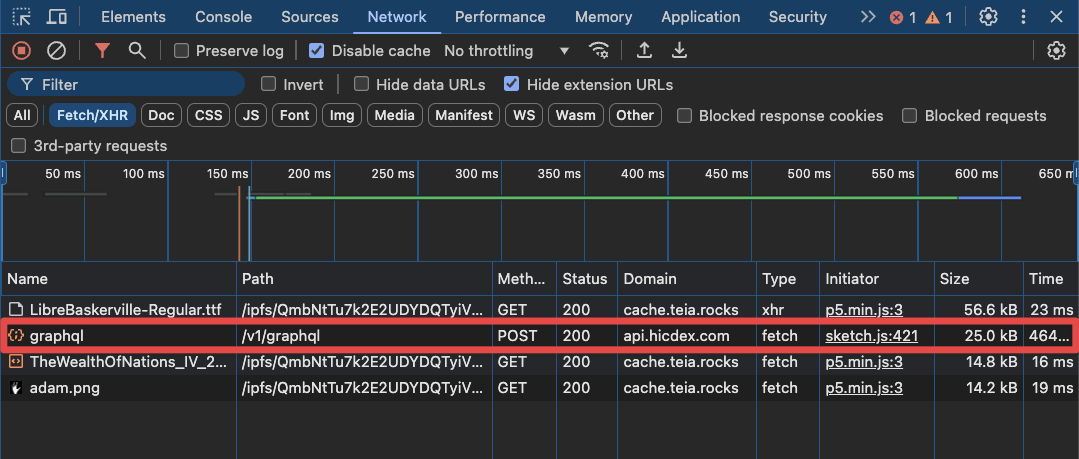
\includegraphics[width=\linewidth]{dev-tools-net.png}
    \caption[Developer Tools - Network Inspection]{Developer Tools - Network Inspection}
    \label{fig:devtools-net}
\end{figure}

Now that we established that we can identify a networked OBJKT manually, the next step is to do it programatically.

At this stage we can start to plan our Miles. The numbers will go up the further we get away from our goal.

Analysing the network traffic and determining if an OBJKT is networked is Mile 1.


For capturing the network traffic programatically we can use one of several headless browser automation solutions, which are normally used for automated website testing and web-scraping, like Playwright\footnotemark[2], Selenium\footnotemark[3], or Puppeteer\footnotemark[4]. For this work Playwright was selected. This is Mile 2.


\footnotetext[2]{https://playwright.dev/}
\footnotetext[3]{https://www.selenium.dev/}
\footnotetext[4]{https://pptr.dev/}

Although our Playwright instance could access the OBJKT asset directly from the Teia IPFS node, there are several reasons why it's not desirable to do so:

\begin{enumerate}
	\item introduces potential network latency which could affect the snapshot process adversely
	\item increases the bandwidth usage between teia and arkivo
	\item arkivo is supposed to archive these artworks anyway, including full copies of the assets
\end{enumerate}

For this reason the next step is to run our own IPFS node, so that we can fetch the OBJKTs locally, and pin them, which ensured it cannot be garbage collected by the node. This is Mile 3.

But this raises another question, which artworks to fetch? We need a way to discover and index all the OBJKTs that we are interested in investigating. This is Mile 4.

To discover the OBJKTs we can resort to existing indexers of the Tezos blockchain. There are 2 main options:

\begin{enumerate}
	\item TzKT API\footnotemark[5] - a generic indexer for the whole Tezos blockchain
	\item TezTok API\footnotemark[6] - an indexer specialised in Tezos NFTs
\end{enumerate}

\footnotetext[5]{https://tzkt.io/api}
\footnotetext[6]{https://www.teztok.com}

The TzKT API being generic, operates at a very low level, with endpoints that are closely related to the blockchain data, without abstraction layers.
TezTok, on the other hand, specialises in NFTs so it creates an abstraction layer that is easier to work with, since it is NFTs we are interested in discovering. For this reason TezTok was chosen.

Finally, we can move to the last stage, determining what search criteria to use when querying Teztok. This is Mile 5.

Here is a summary of the five Miles. We will write them in the reverse order, as now we are going back towards our goal.

\vspace{0.5cm}

\begin{table}[h]
\footnotesize
\centering
\begin{tabular}{|c|p{10cm}|}
\hline
\textbf{Mile} & \textbf{Description} \\ \hline
Mile 5 & Determine search criteria to use in Mile 4 \\ \hline
Mile 4 & Query TezTok to identify which artworks to fetch (discovery) \\ \hline
Mile 3 & Fetch and pin all OBJKTs of potential interest \\ \hline
Mile 2 & Run OBJKT in Playwright sandbox and capture traffic \\ \hline
Mile 1 & Analyse traffic and determine if the OBKJT is networked \\ \hline
\end{tabular}
\caption{The 5 Miles of Development for RQ1}
\end{table}

With these in place we draft an iteration plan. This can always be changed later but will give a rough idea of how many iterations are required.


\begin{table}[h]
\footnotesize
\centering
\begin{tabular}{|l|c|l|}
\hline
\textbf{Iteration}        & \multicolumn{1}{l|}{\textbf{Mile}} & \textbf{Description}                                         \\ \hline
\multirow{2}{*}{Iteration RQ1.1} & Mile 5                              & Determine search criteria to use in Mile 4                   \\ \cline{2-3} 
                             & Mile 4                              & Query TezTok to identify which artworks to fetch (discovery) \\ \hline
Iteration RQ1.2                  & Mile 3                              & Fetch and pin all OBJKTs of potential interest               \\ \hline
\multirow{2}{*}{Iteration RQ1.3} & Mile 2                              & Run OBJKT in Playwright sandbox and capture traffic          \\ \cline{2-3} 
                             & Mile 1                              & Analyse traffic and determine if the OBKJT is networked      \\ \hline
\end{tabular}
\caption{Iteration Plan for RQ1}
\end{table}



\section {Iteration RQ1.1}


\begin{table}[H]
\footnotesize
\centering
\begin{tabular}{|l|c|l|}
\hline
\textbf{Iteration}        & \multicolumn{1}{l|}{\textbf{Mile}} & \textbf{Description}                                         \\ \hline
\multirow{2}{*}{Iteration RQ1.1} & Mile 5                              & Determine search criteria to use in Mile 4                   \\ \cline{2-3} 
                             & Mile 4                              & Query TezTok to identify which artworks to fetch (discovery) \\ \hline
\end{tabular}
\caption{Iteration RQ1.1 Miles}
\end{table}


\subsection {Mile 5}

Mile 5 is really just an exploratory phase, which does not require any development. It involves accessing Teztok's GraphQL playground\footnotemark[7], exploring the schema available, and crafting a query that returns a list of OBJKTs of interest.

\footnotetext[7]{https://graphiql.teztok.com/}

We want all OBJKTs of mime-type \texttt{application/x-directory} and \\ \texttt{image/svg+xml} from the HEN OBJKT smart contract \\\texttt{KT1RJ6PbjHpwc3M5rw5s2Nbmefwbuwbdxton} and we select all the metadata fields that are interesting to us, including \texttt{artifact\_uri} which is the CID of the OBJKT media asset in the IPFS network.


\vspace{0.5cm}

\begin{lstlisting}[language=HTML, caption={GraphQL query to retrieve OBJKTs of interest}] 
query artifact_metadata {
  tokens(where: {_or: [{mime_type: {_eq: "application/x-directory"}},
    									 {mime_type: {_eq: "image/svg+xml"}}],
    						 fa2_address: {_eq: "KT1RJ6PbjHpwc3M5rw5s2Nbmefwbuwbdxton"}},
    						 order_by: {minted_at: asc}, offset: 0, limit: 10) {
    token_id
    name
    artifact_uri
    metadata_uri
    thumbnail_uri
    mime_type
    description
    tags {
      tag
    }
    artist_address
    fa2_address
    platform
    minted_at
    editions
  }
}
\end{lstlisting}


Following is a sample of a record returned by this query:


\vspace{0.5cm}

\begin{lstlisting}[language=HTML, caption={Sample OBJKT Record }] 

"tokens": [
      {
        "token_id": "229",
        "name": "The Bird",
        "artifact_uri": "ipfs://QmUHJdbFukpVBSqVnQ7V1C9JEFR5XC2pFZW17LUEpAtQnd",
        "metadata_uri": "ipfs://QmbaWzPvtJJXJT8bqxUrFUQkraV3uHV4rzrXFLBcJ18kH1",
        "thumbnail_uri": "ipfs://QmNrhZHUaEqxhyLfqoq1mtHSipkWHeT31LNHb1QEbDHgnc",
        "mime_type": "image/svg+xml",
        "description": "The Bird. SVG. 2021. @djangobits",
        "tags": [],
        "artist_address": "tz1YRG68NdqtAcsFEwTUw6FsSsiBb5kagEDo",
        "fa2_address": "KT1RJ6PbjHpwc3M5rw5s2Nbmefwbuwbdxton",
        "platform": "HEN",
        "minted_at": "2021-03-02T06:16:35+00:00",
        "editions": 1
      },
   [snip]
\end{lstlisting}




\subsection {Mile 4}

Mile 4 is the beginning of development, and because it's the first we need to a barebones application. For this project the AdonisJS web framework was selected as the stack for the application, because it provides a full-stack MVC Framework, supports TypeScript, and follows a convention over configuration environment which helps speed up development. It also provides a very convenient way to create \indexacronym{cli} commands that we can use to control aspects of our application, such as starting batch jobs, or triggering specific actions.

In this Mile we need to:

\begin{enumerate}
	\item Query TezTok and receive the list of OBJKTs. Because the listing is very large, we need to paginate the results with the use of the \texttt{limit} and \texttt{offset} parameters in the query
	\item Store each OBJKT metadata in a local Postgres database, which will serve as the main database of our application.
\end{enumerate}



\begin{figure}[h]
    \centering
    \includesvg[width=0.75\textwidth]{mile4-arch}
    \caption[Mile 4 Architecture]{Mile 4 Architecture}
    \label{fig:mile4-arch}
\end{figure}


This concludes iteration RQ1.1. At this stage our database contains the metadata of 21,390 OBJKTs.


\section {Iteration RQ1.2}
\label{sec:rq1.2}

\begin{table}[h]
\footnotesize
\centering
\begin{tabular}{|l|c|l|}
\hline
\textbf{Iteration}        & \multicolumn{1}{l|}{\textbf{Mile}} & \textbf{Description}                                         \\ \hline
Iteration RQ1.2                  & Mile 3                              & Fetch and pin all OBJKTs of potential interest               \\ \hline
\end{tabular}
\caption{Iteration RQ1.2 Mile}
\end{table}


\subsection {Mile 3}

In this Mile we will start pinning the OBJKTs assets in a local IPFS node. This is a significant milestone because from this moment onwards, the system is already delivering a useful service to the ecosystem. By pinning content and participating in the IPFS p2p network we are helping other nodes access the content.

Tasks for Mile 3:
\begin{enumerate}
	\item Setup an IPFS node (Kubo)\footnotemark[8] to fetch and pin the OBJKTs
	\item For each OBJKT metadata, we instruct the IPFS node to pin the CIDs of that OBJKT. This operation will also automatically fetch the assets to the IPFS node. These operations take a significant amount of time, so we need to queue the operations in a Redis database, which is consumed by a worker that actually communicates with the IPFS node.
\end{enumerate}

\footnotetext[8]{https://github.com/ipfs/kubo}



\begin{figure}[h]
    \centering
    \includesvg[width=0.75\textwidth]{mile3-arch}
    \caption[Mile 3 Architecture]{Mile 3 Architecture}
    \label{fig:mile3-arch}
\end{figure}


After all OBJKTs are fetched and pinned, the IPFS node is using 79.3GB of disk size.

\label{txt:rq3-answered}
And just like that, Iteration RQ1.2 answered RQ3:

\vspace{0.5cm}
RQ3 - What are the disk space requirements for storing all code-based HEN OBJKTs’ media assets?
\vspace{0.5cm}

\section {Iteration RQ1.3}


\begin{table}[h]
\footnotesize
\centering
\begin{tabular}{|l|c|l|}
\hline
\textbf{Iteration}        & \multicolumn{1}{l|}{\textbf{Mile}} & \textbf{Description}                                         \\ \hline
\multirow{2}{*}{Iteration RQ1.3} & Mile 2                              & Run OBJKT in Playwright sandbox and capture traffic          \\ \cline{2-3} 
                             & Mile 1                              & Analyse traffic and determine if the OBKJT is networked      \\ \hline
\end{tabular}
\caption{Iteration RQ1.3 Miles}
\end{table}



\subsection {Mile 2}

In this Mile we will use PlayWright to open each OBJKT and record any network calls initiated by the OBJKT. This is done in \texttt{SnapshotArtifactService}

Tasks for Mile 2:
\begin{enumerate}
	\item Run each OBJKT in a Playwright sandbox and capture traffic, including URLs and any payloads
\end{enumerate}



\begin{figure}[h]
    \centering
    \includesvg[width=0.9\textwidth]{mile2-arch}
    \caption[Mile 2 Architecture]{Mile 2 Architecture}
    \label{fig:mile2-arch}
\end{figure}


Snapshots take a significant amount of time, because each snapshot must wait for a few seconds in case an OBJKT makes late network calls. For this reason \texttt{ProcessArtifact} had to be run on two different node processes, each one consuming from a separate Redis queue: \texttt{ipfs} and \texttt{snapshots}.

A significant issue was found at this Mile: the PlayWright library does not release resources when a browser instance is closed, which causes a memory leak after only a short amount of time doing continuous snapshots. This is a known issue, and unlikely to be fixed soon. For this reason, the \texttt{ProcessArtifact} process in charge of snapshots must force exit itself after only 5 snapshots, and do this while wrapped in a shell-script which automatically restarts it each time. This way all resources are freed, every 5 snapshots.


\vspace{0.5cm}

\begin{lstlisting}[language=bash, caption={runSnapshotWorker.sh}] 
#!/bin/bash

# Infinite loop to restart the command whenever it exits
while true; do
  # Execute the Node.js command
  node ace queue:listen --queue=snapshot

  # Wait for a second before restarting to avoid spamming in case of immediate failure
  sleep 1
done
\end{lstlisting}


\subsection {Mile 1}

At this stage we code the logic that checks whether an OBJKT makes external network requests, and when it does, record that in a \texttt{is\_networked} database field.

Tasks for Mile 1:
\begin{enumerate}
	\item Analyse traffic and determine if the OBKJT is networked
\end{enumerate}


After completing this process, we can query the database to find how many OBJKTS are networked. We do want to exclude those which have been burned, or destroyed by their creators, which are normally failed or test mints.

\begin{center}
\begin{lstlisting}[language=SQL, caption={SQL query - number of networked OBJKTs}]
SELECT COUNT(id)
FROM artifacts
WHERE is_networked = true
AND is_burned = false;
\end{lstlisting}
\end{center}

As of this writing, there a total of \texttt{1083} networked OBJKTs on the HEN smart contract and each one is properly labelled in our database. RQ1 has been answered.


\section{Plan for RQ2}

We will now turn our attention to RQ2:

\vspace{0.5cm}
RQ2 - Can we capture and document networked HEN OBJKTs aesthetic evolution?
\vspace{0.5cm}


This question is more difficult to answer because we need to define what we mean by ``aesthetic evolution''. At its most simplistic level, the regular capturing of screenshots of the artwork might suffice in many instances. But artworks which are animated require a different approach, like a video recording. Others might be user interactive, and require yet a different strategy, see \autoref{subsec:capture-interactive}. External elements, like artist, curator, and conservator documentation, audience reactions, and many others, could also be considered a part of an artwork's aesthetic evolution. All these would require in-depth classification and analysis of the artwork, which is not feasible within the timeframe of this project. Therefore the scope will be reduced to the content delivered within the OBJKT's canvas. Also, having in mind the economic sustainability of the project, the decision was made to only take a static screenshot of the artwork during a snapshot to keep the storage space requirements to a minimum.


\begin{table}[h]
\footnotesize
\centering
\begin{tabular}{|l|c|l|}
\hline
\textbf{Iteration}        & \multicolumn{1}{l|}{\textbf{Mile}} & \textbf{Description}                                         \\ \hline
Iteration RQ2.1                  & Mile 1                              & Take screenshot of OBJKT during snapshot               \\ \hline
\end{tabular}
\caption{Iteration Plan for RQ2}
\end{table}

\section {Iteration RQ2.1}


\subsection {Mile 1}

Since we already have our snapshotting infrastructure in place, all we need is to take a screenshot at the end of the snapshotting process and store it. For now we will store the screenshots as base64-encoded PNGs in our snapshot record. This is not ideal in the long term, as the database will grow quite rapidly, but it works for the purposes of our research question, and that is all that is required when following the RQDD method.

\autoref{lst:screenshotcode} shows an abbreviated version of the code which takes the screenshot, using the PlayWright library.

\vspace{0.5cm}

\begin{lstlisting}[language=JavaScript, caption={OBKJT screenshot code}, label={lst:screenshotcode}] 

async snapshot(artifact: Artifact, dryRun: boolean): Promise<void> {

  const START_TIME = Date.now();

  // strip ipfs prefix from url
  let url = artifact.artifactUri;
  const pageUrl = this.formatPlatformUrl(artifact, url);

  // prepare browser instance
  const browser = await chromium.launch();
  const context = await browser.newContext({
      viewport: { width: DEFAULT_VIEWPORT_WIDTH,
                  height: DEFAULT_VIEWPORT_HEIGHT
                }
  });

  // open artifact URL
  const page = await context.newPage();
  await page.goto(pageUrl);

  // wait for the remaining time
  const TIME_LEFT = SNAPSHOT_DURATION - (Date.now() - START_TIME);
  await page.waitForTimeout(TIME_LEFT);

  // capture screenshot
  console.log(`Taking screenshot...`);
  const buffer = await page.screenshot({ timeout: 60000 });
  this.snapshotData.snapshot.screenshot = buffer.toString('base64');
\end{lstlisting}

After a round of snapshots with screenshots across all the OBJKTs indexed in our database, the \texttt{snapshots} table grew significantly in size, as expected: 26GB. The total database size, including the OBJKTs metadata, is 29.4GB.

A sample of screenshots was manually inspected, and all worked as expected. Later we will develop a web UI where the screenshots can be easily inspected.

This first snapshot is important, as it is used for the initial classification of the OBJKT (networked or not), as well as to establish a baseline record, against which future snapshots can be compared. Therefore it should be taken immediately after discovery/ingestion of new OBJKTs.

This feature allows us to capture screenshots of each OBJKT across time, which answers RQ2, even if in the limited scope that we discussed above.

\section{Plan for RQ3}

RQ3 was answered by Iteration RQ1.2, see \autoref{sec:rq1.2}, page \pageref{txt:rq3-answered}.

\section{Plan for RQ4}

RQ4 is the most challenging of all our research questions:

\vspace{0.5cm}
RQ4 - Can an online archive for HEN OBJKTs be economically self-sustainable?
\vspace{0.5cm}

To answer this question we need to understand what are the recurring costs of running such an archive, so that we can calculate the amount of income required to break-even, and then determine if such a source of income can be sustained and how.

Even though this requires mostly a financial analysis, there is a component of development that is required: to create and host an actual online archive.
The application developed for the previous RQs already suffices as a backend for such an archive, so all we need is to develop a web-interface that allows for the browsing and searching of the artworks.

Once deployed in production we will determine the recurring cost of hosting the system which will allow us to proceed with the break-even analysis.

This RQ only requires one iteration.

\section {Iteration RQ4.1}

\begin{table}[H]
\footnotesize
\centering
\begin{tabular}{|l|c|l|}
\hline
\textbf{Iteration}        & \multicolumn{1}{l|}{\textbf{Mile}} & \textbf{Description}                                         \\ \hline
\multirow{2}{*}{Iteration RQ4.1} & Mile 2                              & Develop web UI                   \\ \cline{2-3} 
                             & Mile 1                              & Deploy system in production \\ \hline
\end{tabular}
\caption{Iteration RQ4.1 Miles}
\end{table}

\subsection {Mile 2}

To develop the web UI we start by sketching a basic wireframe to plan the layout of the pages. We only need 2 page templates, one for browsing the OBJKTs and another to display a particular OBJKT, see \autoref{fig:web-wireframe}.
The browsing page will display 9 artworks at once, with a page navigation control at the bottom.
The detail page is somewhat inspired in the Rhizome ArtBase website, with the inclusion of the accordion menus, to show and collapse the details about the artwork.

\begin{figure}[H]
  \centering
  \begingroup
  \setlength{\fboxsep}{0pt} % No padding between box and content
  \setlength{\fboxrule}{1pt} % Thickness of the border
  \begin{subfigure}[b]{0.45\textwidth}
    \centering
    \fcolorbox{gray}{white}{\includesvg[width=\textwidth]{wireframe-browse.svg}}
    \caption{Artifact Browsing Page}
    \label{fig:wireframe1}
  \end{subfigure}
  \hfill
  \begin{subfigure}[b]{0.45\textwidth}
    \centering
    \fcolorbox{gray}{white}{\includesvg[width=\textwidth]{wireframe-objkt.svg}}
    \caption{Artifact Detail Page}
    \label{fig:wireframe2}
  \end{subfigure}
  \endgroup
  \caption{Artifact Web UI Wireframe}
  \label{fig:web-wireframe}
\end{figure}

With the overall UI mapped out, it was just a matter of coding it, using AdonisJS Edge templating engine. In the Artifact Detail Page, we can see one of the snapshots for the artwork, including the screenshot of the artwork.

For the search facility, a checkbox was added to optionally restrict the search to networked OBJKTs only. This makes use of the automatic classification of networked OBJKTs developed in Iteration RQ1.3 Mile 1.

\begin{figure}[H]
  \centering
  \begingroup
  \setlength{\fboxsep}{0pt} % No padding between box and content
  \setlength{\fboxrule}{1pt} % Thickness of the border
  \begin{subfigure}[b]{0.45\textwidth}
    \centering
    \fcolorbox{gray}{white}{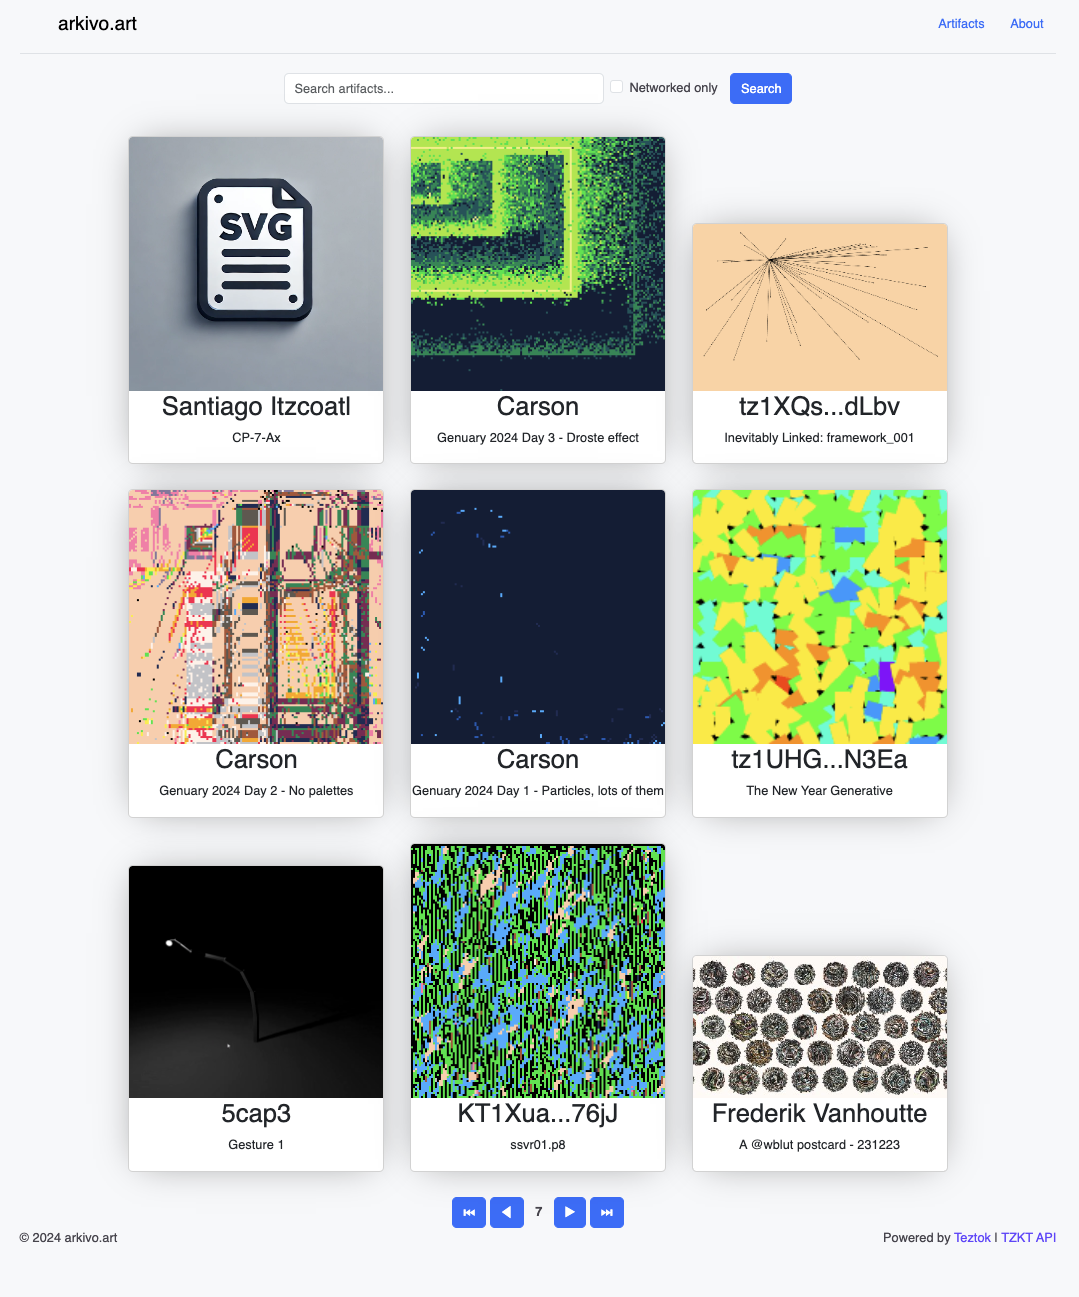
\includegraphics[width=\textwidth]{arkivo-ui-browse.png}}
    \caption{Artifact Browsing Page}
    \label{fig:wireframe1}
  \end{subfigure}
  \hfill
  \begin{subfigure}[b]{0.45\textwidth}
    \centering
    \fcolorbox{gray}{white}{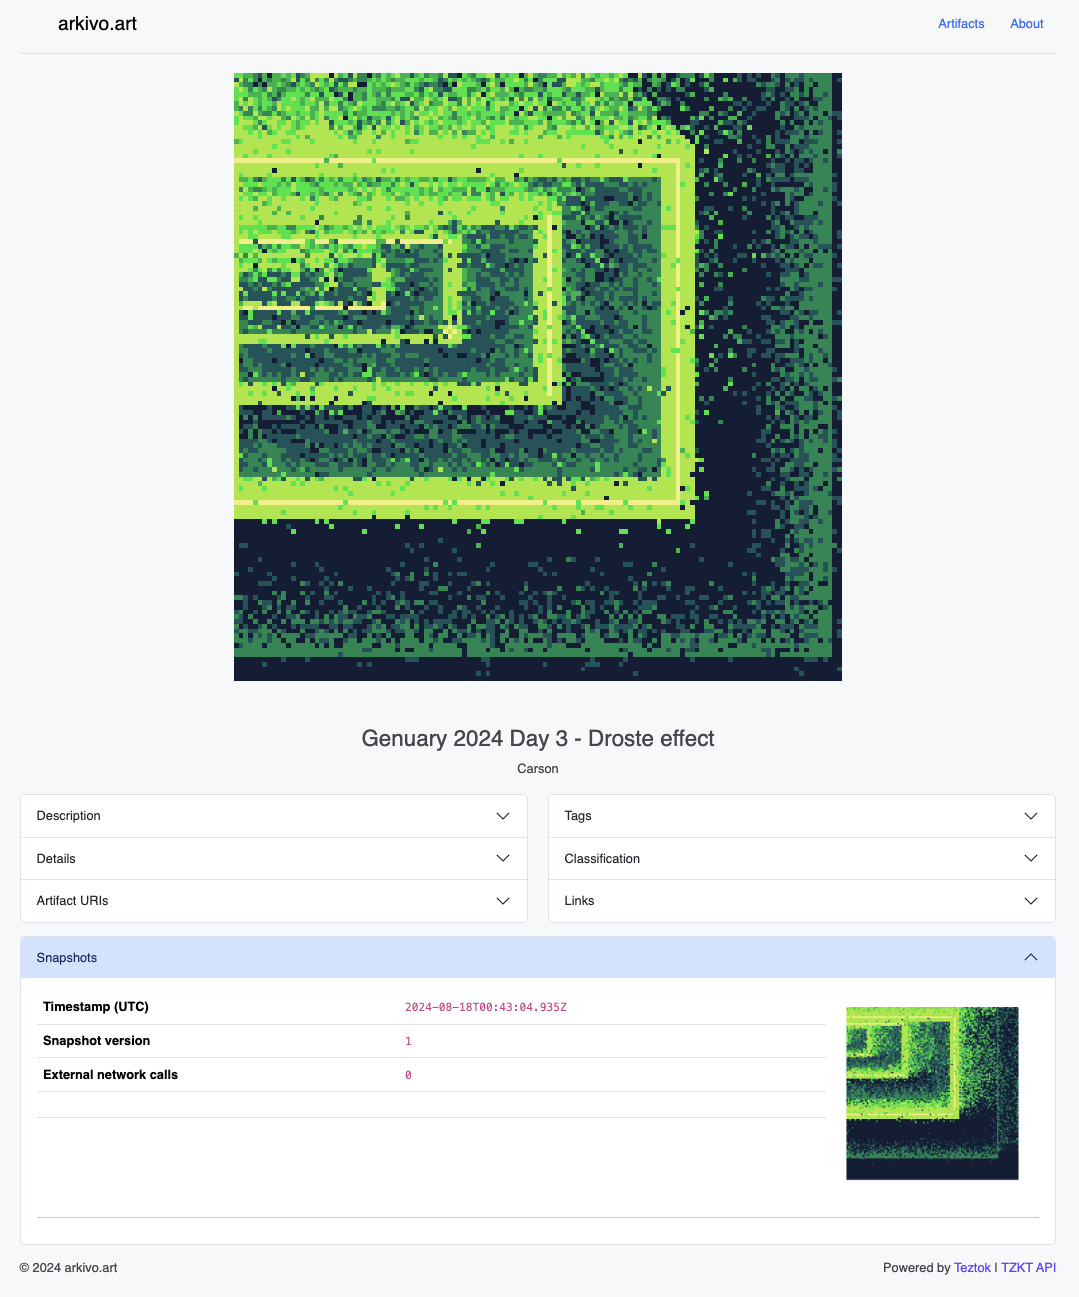
\includegraphics[width=\textwidth]{arkivo-ui-detail.png}}
    \caption{Artifact Detail Page}
    \label{fig:wireframe2}
  \end{subfigure}
  \endgroup
  \caption{Artifact Web UI Implementation}
  \label{fig:web-implementation}
\end{figure}

Also a basic "About" page was created, with a short description of what the project is about. This page also acts as the landing page when a user accesses the main site URL.

\begin{figure}[H]
    \centering
    \begingroup
    \setlength{\fboxsep}{0pt} % No padding between box and content
    \setlength{\fboxrule}{1pt} % Thickness of the border
    \fcolorbox{gray}{white}{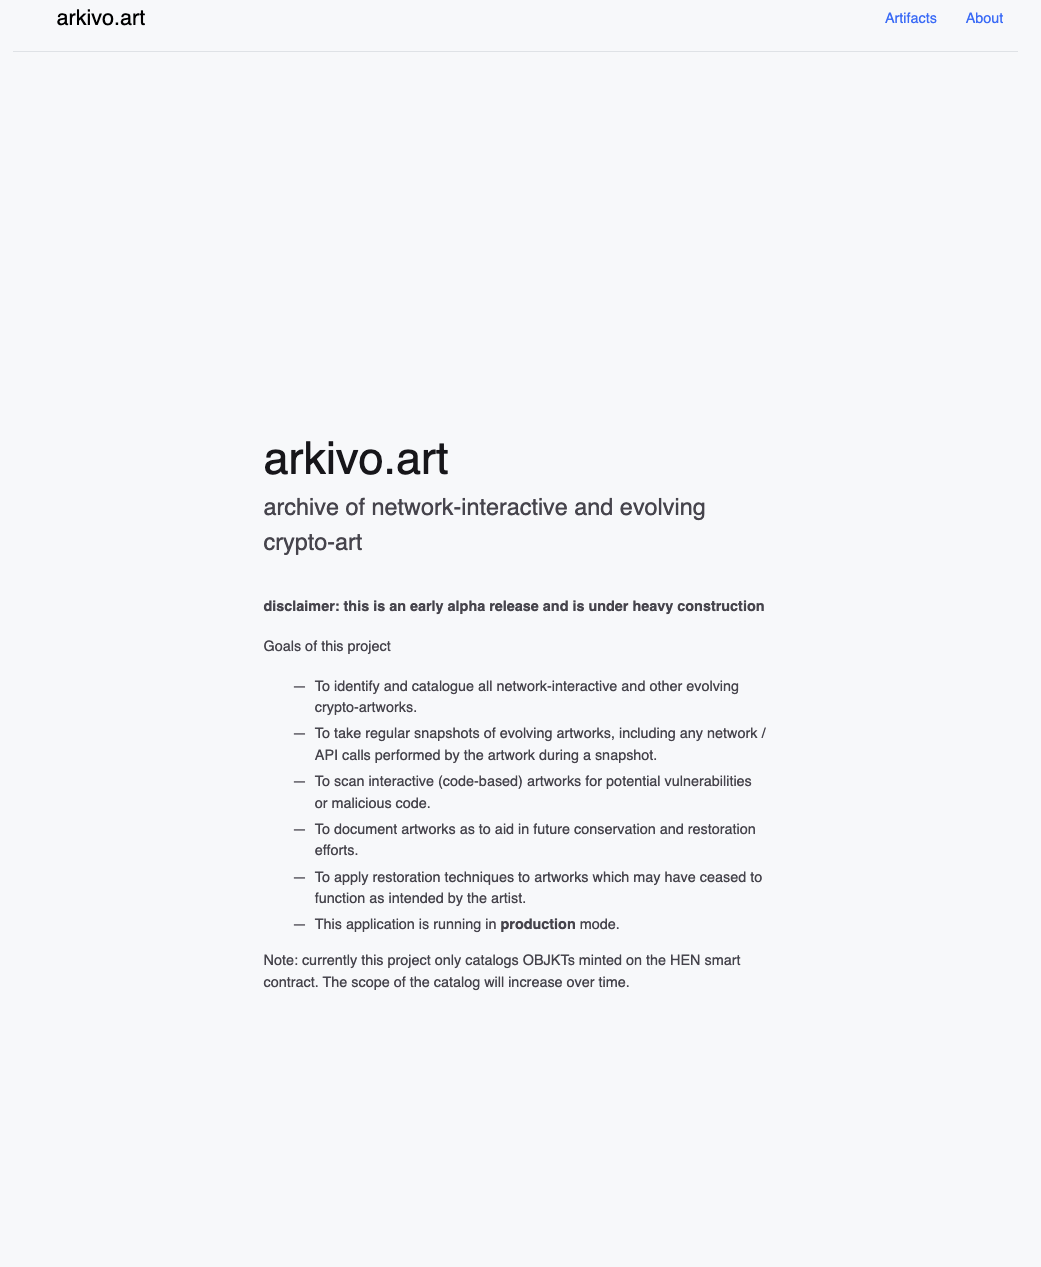
\includegraphics[width=0.75\linewidth]{arkivo-landing.png}}
    \endgroup
    \caption[About Page]{About Page}
    \label{fig:about-page}
\end{figure}



The completion of this Mile signals the end of the development phase of this project.

\subsection {Mile 1}

To deploy the system in production first we need to select a virtual private server (\indexacronym{vps}) hosting company that is reasonably priced for our storage needs. The calculation is based on the disk space used in our testing environment.

\begin{table}[h]
\footnotesize
\centering
\begin{tabular}{|l|r|}
\hline
\textbf{Description} & \textbf{Space Required (GB)} \\ \hline
IPFS                 & 79.0                         \\ \hline
Database             & 29.4                         \\ \hline
\textbf{Total}       & \textbf{108.4}               \\ \hline
\end{tabular}
\caption{\texttt{ARKIVO} Storage Requirements}
\label{table:storage-req}
\end{table}


As we can see from \autoref{table:storage-req}, the test instance of our application is using just under 110GB of disk space. Therefore we need to look for a virtual server with 150GB or more of space, to have some spare margin.

After evaluating a number of hosting options, Hetzner\footnotemark[9] was found to offer the most reasonably priced virtual servers, so it was chosen as the hosting provider for \texttt{ARKIVO}.
The CX42 option was selected, which provides the required space, and offers 16GB of RAM, which allows for more caching of assets in RAM when serving content. The cost of this server is EUR 15.90 per month.

\footnotetext[9]{https://www.hetzner.com/cloud/}

\begin{figure}[H]
    \centering
    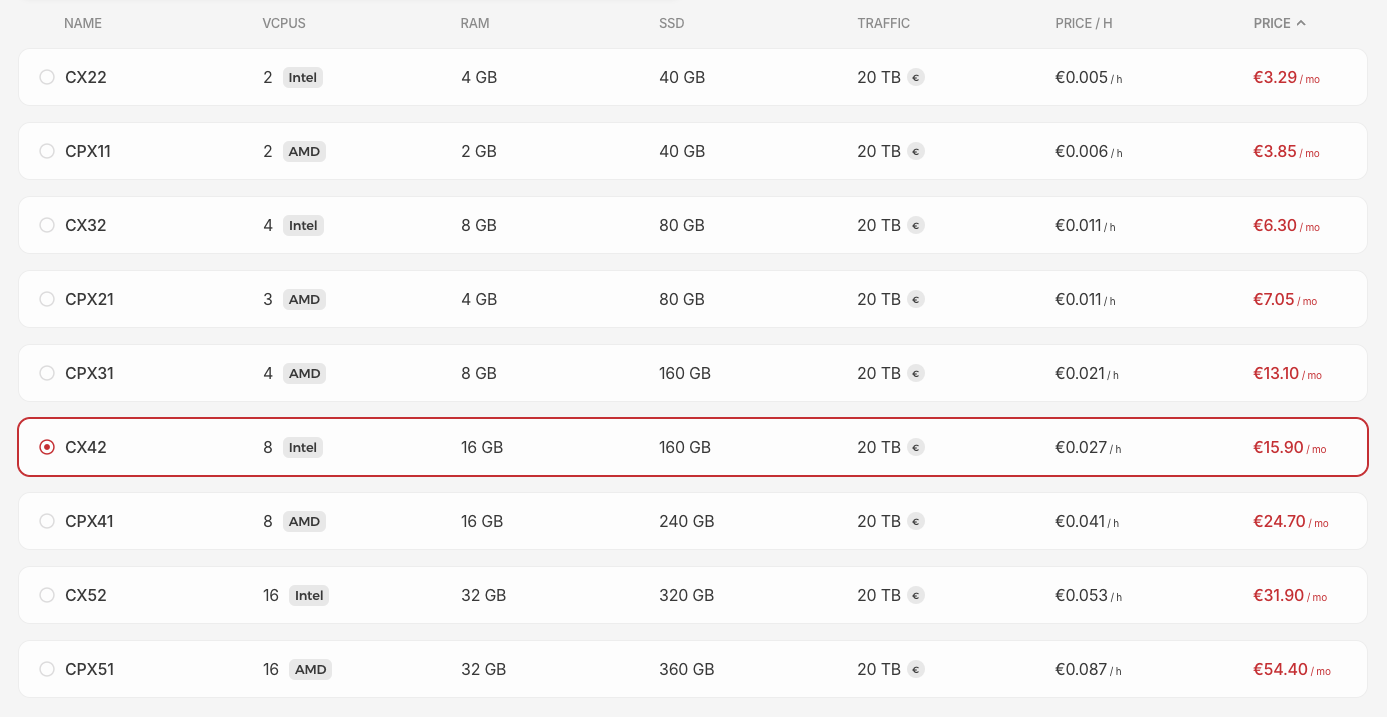
\includegraphics[width=\linewidth]{virtual-server-price.png}
    \caption[Choice of Virtual Server]{Choice of Virtual Server}
    \label{fig:vps-choice}
\end{figure}

The application was successfully installed, using Docker containers for all components. An ngnix webserver docker container acts as a reverse proxy for the main app and for the IPFS node, and it also handles SSL termination. The SSL certificate was acquired by using the Let's Encrypt Certbot.

\begin{figure}[h]
    \centering
    \includesvg[width=0.75\textwidth]{vps-docker.svg}
    \caption[Docker Containers]{Docker Containers}
    \label{fig:docker-containers}
\end{figure}

Note: at the time of writing, in addition to ports 80 and 443, ngnix is also forwarding port 8080 to the app. This is a temporary requirement as if facilitates ``hot-fixes'' without the need for code re-deployment, which is useful during this early stage of development.

\vspace{0.5cm}

\texttt{ARKIVO} is live and accessible at: \texttt{https://arkivo.art/}


\section{Database Schema}

There are 5 main tables in the database schema:

\begin{enumerate}
	\item \texttt{artifacts} - the main table for storing the artifact metadata
	\item \texttt{snapshots} - contains all the snaphots taken. It has a one-to-many relationship with \texttt{artifacts}
	\item \texttt{origins} - contains all the origins (\texttt{schema, domain, port}) that artifacts connect to. It has a many-to-many relationship with \texttt{artifacts}, using a pivot table \texttt{artifact\_origin}
	\item \texttt{tags} - contains all the tags used by artifacts. It has a many-to-many relationship with \texttt{artifacts}, using a pivot table \texttt{artifact\_tag}
	\item \texttt{identities} - contains metadata about artists. It should have a many-to-many relationship with \texttt{artifacts}, but this was postponed for a future iteration as handling multiple artist OBJKTs (collabs) will require work that is outside the scope of this thesis.
\end{enumerate}

There are also 2 additional tables \texttt{adonis\_schema} and \texttt{adonis\_schema\_versions} which are used by AdonisJS to manage database schema migrations, and not relevant for this thesis.

The Entity Relationship Diagram is illustrated in \autoref{fig:db-entity-relationship}.


\begin{figure}[H]
    \centering
    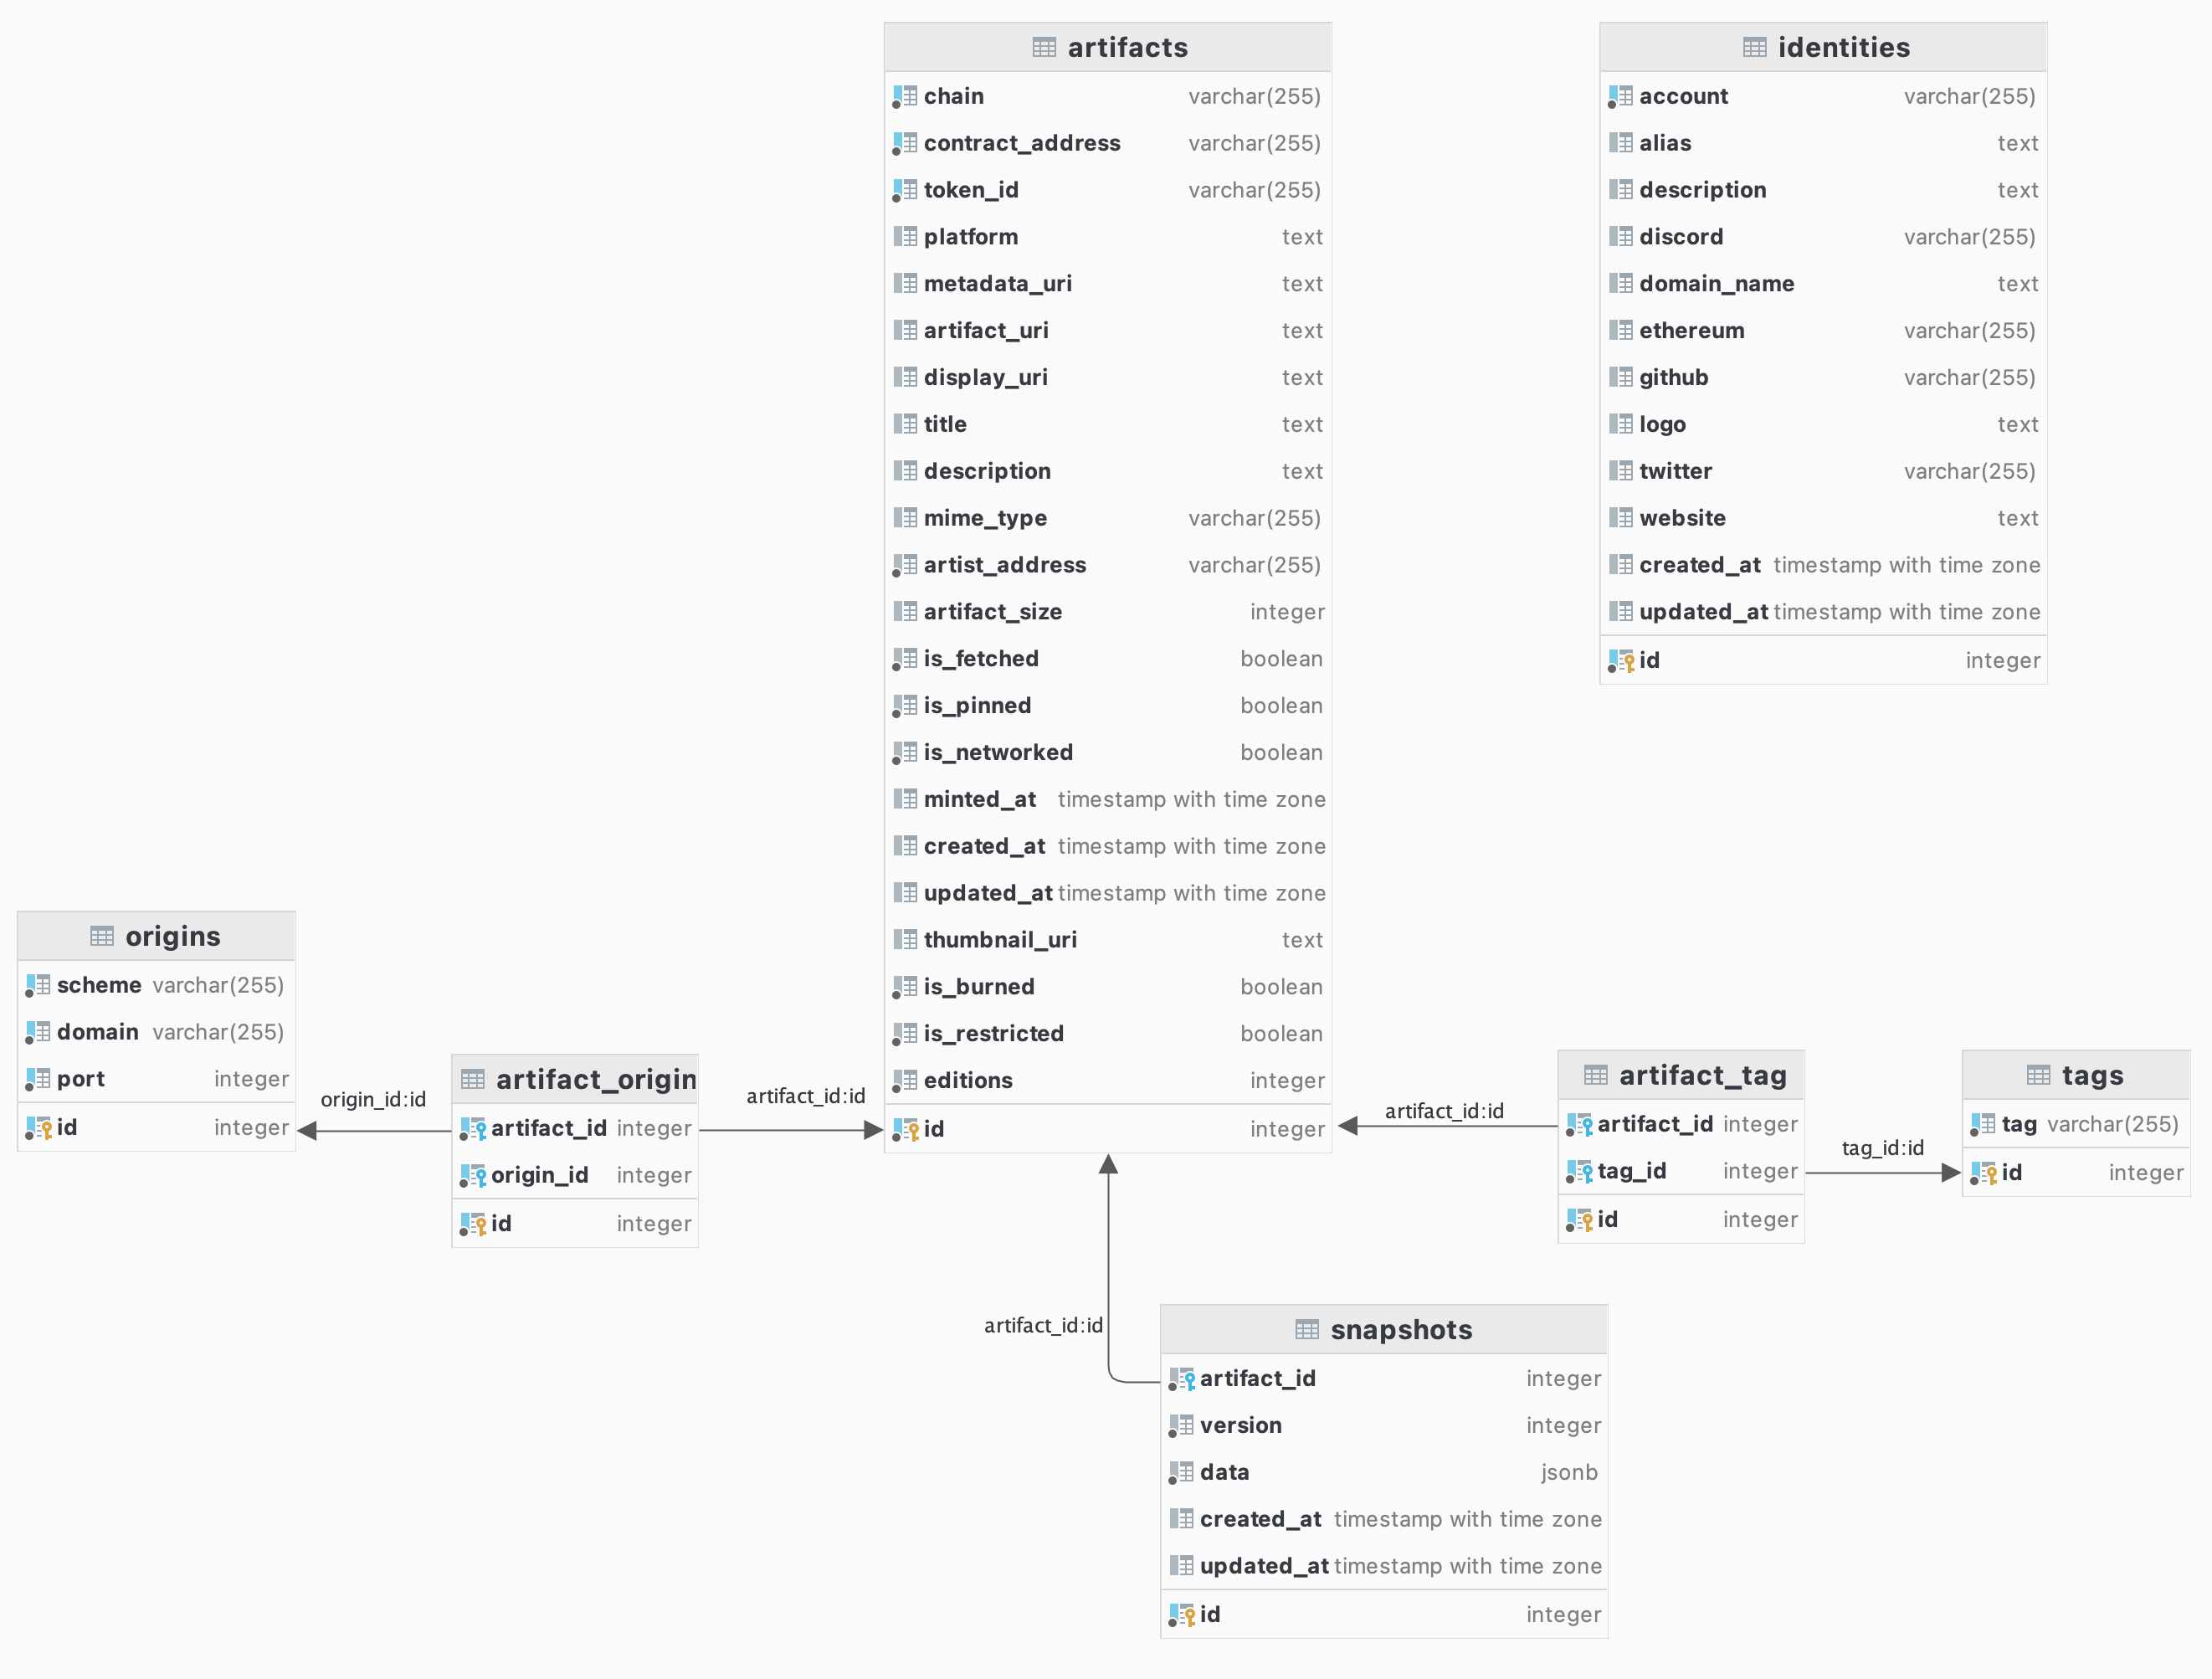
\includegraphics[width=\linewidth]{arkivo_schema.png}
    \caption[Entity Relationship Diagram]{Entity Relationship Diagram}
    \label{fig:db-entity-relationship}
\end{figure}



\section{Catalogue Management}

Currently the management of the archive's catalogue is all done through CLI on the server, using AdonisJS \texttt{node ace} command facility.
The following commands were created to facilitate the initialisation of a new \texttt{ARKIVO} instance:

{\footnotesize
\begin{verbatim}
artifacts:discover         Discovers new artifacts' metadata from
                           the specified platform, optionally
                           pinning their payloads

artifacts:pin              Fetches and Pins already existing
                           artifacts records

artifacts:snapshot         Take a snapshot of an artifact

artifacts:updateMetadata   Update all token metadata for the
                           specified platform
\end{verbatim}
}



\section{Other Notes on the Artifact}

\subsection{Webpage metadata}

A common issue with most web pages, which can cause considerable annoyance to researchers who are working under tight deadlines, is the fact that they often lack the required metadata that is used by reference management tools, like Zotero, to automatically pull the metadata and populate the bibliographical record.

By default Arkivo suffered from the same problem, so attention was given to resolving this.
The \texttt{ArtifactController} now prepares a special data structure, \texttt{citationMetadata}, with all the required data fields, which is then used by the \texttt{header} section of the Edge template.
After experimenting with different metadata standards \cite{DevExposing_metadataZotero}\cite{zahidOpenGraphMeta2023} , a solution was found using a mixture of standards, where Zotero can pull most of the relevant fields related to an artifact, as shown in \autoref{fig:zotero-metadata-comparison}


\begin{lstlisting}[language=HTML, caption={Artifact page metadata}] 
<title>{{ citationMetadata.title}} - arkivo.art</title>
<meta property="og:title" content="{{ citationMetadata.title }}">
<meta property="og:type" content="website">
<meta property="dc.creator" content="{{ citationMetadata.author }}">
<meta property="article:published_time" content="{{ citationMetadata.date }}">
<meta property="og:description" content="{{ citationMetadata.description }}">
<meta property="og:site_name" content="arkivo.art">
\end{lstlisting}


\begin{figure}[H]
  \centering
  \begin{subfigure}[b]{0.45\textwidth}
    \centering
    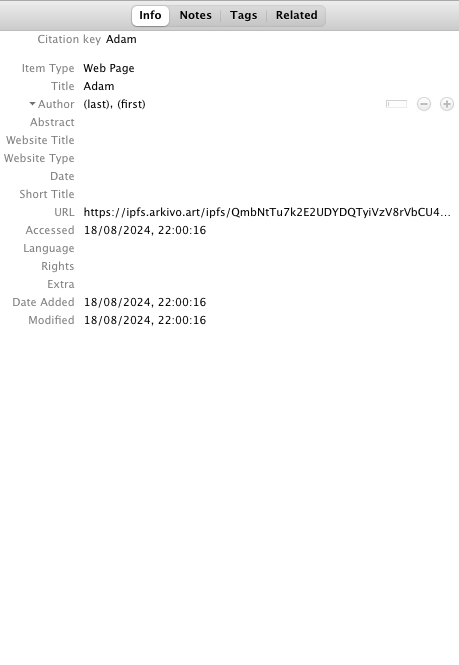
\includegraphics[width=\textwidth]{page-metadata-before.png}
    \caption{Before header metadata}
    \label{fig:image1}
  \end{subfigure}
  \hfill
  \begin{subfigure}[b]{0.45\textwidth}
    \centering
    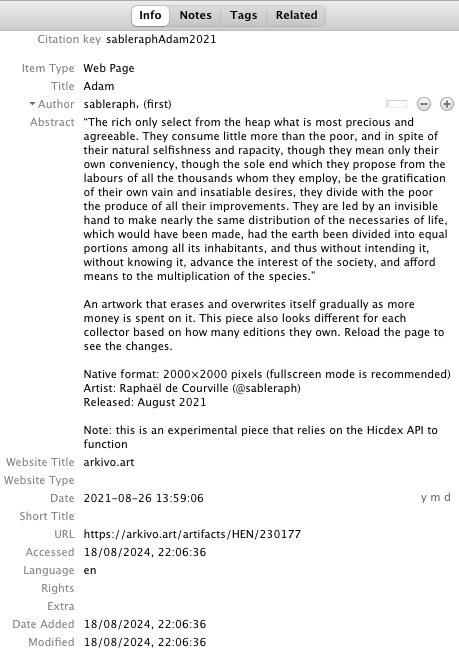
\includegraphics[width=\textwidth]{page-metadata-after.png}
    \caption{After header metadata}
    \label{fig:image2}
  \end{subfigure}
  \caption{Artifact metadata pulled by Zotero}
  \label{fig:zotero-metadata-comparison}
\end{figure}


\subsection{Encapsulation of internal IDs}

In normal circumstances the listing of a model, like Artifact, would include the unique ID of that model as stored in the database, for example: \texttt{/artifacts/45}

However this ID is unique to this instance of the application, and it can change based on the timing of artifact discovery between other instances.
For this reason it is imperative that none of the internal IDs generated by the database are exposed to the user.

In order to achieve this, all URLs must be generated using only public identifiers which uniquely identify a model, in the case of an artifact: \texttt{blockchain /  smart contract / tokenId}.
This scheme closely follows existing proposals for cross-chain standardisation of identifiers \cite{herzogAssetTypeAsset2020}.

So what would be a URL:

\texttt{/artifacts/2065}

Becomes:

\texttt{/artifacts/tezos/KT1RJ6PbjHpwc3M5rw5s2Nbmefwbuwbdxton/230177}


However this URL is quite verbose. For convenience, since most of our initial artifacts are all on tezos, and on the HEN's OBJKT smart contract we can:

\begin{itemize}
    \item omit the blockchain identifier
    \item use an alias for the smart contract address
\end{itemize}

This strategy allows us to have shorter, but still unique URLs, which do not expose our internal DB IDs.

\texttt{/artifacts/HEN/230177}

Even in the cases where a URL is shortened, the long-form URL also works.


\subsection{Open Source License}

This artifact was open sourced under the MIT License.
Open sourcing the project is important because anyone should be able to run an instance and replicate the archive. This follows the philosophy behind web3, which was discussed in Motivation chapter.
















